\documentclass[a4paper,dvipdfm]{article}
\usepackage[margin=1.1in]{geometry}
\usepackage[utf8]{inputenc}
\usepackage[brazil]{babel}
\usepackage{indentfirst}
\usepackage{cite}
\usepackage{url}
\usepackage{graphics}
\usepackage{graphicx}
\usepackage{caption}
\usepackage{subcaption}
\usepackage[acronym]{glossaries}
\usepackage{array}
\usepackage{multirow}
	

\title{Como o spam afeta a comodidade do Correio Eletrônico}
\author{Bianca Madoka Shimizu Oe\\
		Gustavo Shinji Inoue\\
		Rafael Umino Nakanishi}

\makeglossaries

\newacronym{acm}{ACM}{Association for Computing Machinery}
\newglossaryentry{blacklist} {
	name={blacklist}, 
	description={Lista de mensagens classificadas como spam}
}
\newglossaryentry{bot} {
	name={bot}, 
	description={Softwares criados para realizar alguma tarefa de forma automatizada}
}
\newglossaryentry{cabecalho} {
	name={cabeçalho}, 
	description={Parte do e-mail que contem informações suplementares de transmissão. Entre seus campos, são encontrados endereço do emissor, endereço do receptor, endereço de resposta, data de emissão, tipo do conteúdo e assunto}
}
\newglossaryentry{cadmarkov} {
	name={Cadeia de Markov},
	description={Conjunto de estados no qual um processo ocorre. O processo inicia em um estado e se move sucessivamente, transicionando entre estados a cada passo. O estado para o qual o processo se move depende unicamente, de forma probabilística, do estado em que ele se encontra atualmente},
	plural={Cadeias de Markov}
}
\newglossaryentry{captcha} {
	name={CAPTCHA}, 
	description={\emph{Completely Automated Public Turing test to tell Computers and Humans Apart}. Teste criado para diferenciar seres humanos de máquinas. Consiste em imagens de mensagens distorcidas para evitar a interpretação automática por máquinas}
}
\newglossaryentry{crm114} {
	name=\emph{CRM114}, 
	description={Software anti-spam baseado em técnicas estatísticas para a filtragem e classificação de dados. Seu código fonte na linguagem C é disponibilizado sob a licença \emph{GPL}}
}
\newglossaryentry{email} {
	name={e-mail}, 
	description={Correio eletrônico, termo usualmente utilizado para denotar a mensagem eviada por este meio}
}
\newglossaryentry{falsopos} {
	name={falso-positivo}, 
	description={Classificação errônea na qual, para este contexto, um e-mail legítimo é classificado como spam}
}
\newglossaryentry{gpl} {
	name={\emph{GPL}}, 
	description={\emph{General Public License}. Licença para software livre}
}
\newglossaryentry{mta} {
	name={MTA},
	description={Mail Transfer Agent. Software que transfere mensagens de correio eletrônico de um cliente para outro, baseado em uma arquitetura cliente-servidor}
}
\newglossaryentry{oem} {
	name={software OEM},
	description={Produtos ou componentes comprados em grandes lotes a preços menores sob o nome de uma empresa}
}
\newglossaryentry{spambot} {
	name={spambot},
	description={Bot projetado para enviar spam de forma massiva, automaticamente}
}
\newglossaryentry{threshold} {
	name={threshold}, 
	description={Valor utilizado como limitante para uma classificação}
}
\newglossaryentry{whitelist} {
	name={whitelist}, 
	description={Lista de endereços de e-mail de remetentes legítimos, previamente validados}
}

\newcolumntype{C}[1]{>{\centering\let\newline\\\arraybackslash\hspace{0pt}}m{#1}}

\begin{document}
\maketitle
%\newpage

\begin{abstract}
	O uso do correio eletrônico se tornou uma necessidade pessoal com o advento da tecnologia. Com esse novo meio de comunicação há maior praticidade e agilidade na troca de mensagens, de forma que não é necessário se locomover longas distâncias para conversar com outras pessoas.

	Entretanto, a facilidade adquirida também permite o envio de milhares de mensagens eletrônicas em poucos segundos, que podem ser mensagens importantes, como um aviso de uma empresa de grande porte para seus funcionários, ou \emph{spam}, um fenômeno que cresce dia após dia.

	((Mudar isso))
	Nosso objetivo, nesta monografia, é mostrar como o spam vem trazendo inconveniências os usuários de \gls{email}.
	Mostraremos a origem da palavra e seus usos nos dias atuais. 
	((colocar algo como em seguida aqui)) métodos utilizados para separar mensagens importantes de spam.
	Em seguida, alguns exemplos de como esse tipo de mensagem traz desconforto para quem o recebe. 
	Por fim, um estudo de caso, analisando as violações dos códigos da \gls{acm}~\cite{ACM} e a conclusão.
\end{abstract}

\newpage

\tableofcontents
\newpage


\section{Introdução}
	Nesta seção será feita uma breve descrição de como o termo spam (para falar de mensagens indesejadas) foi originado, seguida de ((blablabla)).

	\subsection{Origem do termo}
		A aparição da palavra Spam que originou sua utilização atual ocorreu no episódio 12 da segunda temporada de uma série britânica de comédia chamada \emph{Monty Python's Flying Circus}. 
		Spam é uma mistura de carnes de porco apimentadas e enlatadas, vindo de \emph{SPiced hAM} (Figura \ref{fig:spam}), criado pela empresa estadunidense \emph{Hormel Foods Corporation}.

		Durante o episódio, personagens discutem sobre o cardápio de um café. 
		A carne enlatada é um ingrediente presente em todos os pratos do estabelecimento, sendo considerada algo indesejável por um dos personagens, e, durante a discussão, ``Spam'' foi dito mais de 50 vezes em menos de 4 minutos.

		Apesar de não se saber ao certo quando o termo começou a ser utilizado para denotar mensagens indesejadas, atualmente ele é vastamente utilizado, principalmente para  se referir a e-mails de propagandas inconvenientes.
		
		\begin{figure}[ht]
			\centering
			
\includegraphics [height=5cm]{Imagens/spam/spam.png}
			\caption{Lata de presunto apimentado}
			\label{fig:spam}
		\end{figure}

	\subsection{Spam ((na atualidade))}
		A empresa especializada em segurança \emph{M86 Security Labs}~\cite{m86} separa spam em 13 categorias listadas abaixo:
		\begin{description}
			\item [Fraude] Seu objetivo é fazer o destinatário acreditar que ganhou algo, como um prêmio.
			\item [Adulto] Possui conteúdo pornográfico e oferece cadastro gratuito a \emph{sites} adultos ou a serviços de acompanhantes.
			\item [Financeiro] É relacionado a financiamentos e oferecimento de crédito falso.
			\item [Ações] Anuncia ações de empresas para causar o aumento do preço das mesmas.
			\item [Farmacêuticas] Informa sobre vários tipos de drogas e remédios, geralmente promete uma pele melhor, mais energia, perda de peso, entre outros. 
			Como um exemplo, tem-se o Viagra.
			\item [Phishing] Tenta imitar e-mails legítimos enviados por empresas para conseguir dados e/ou credenciais de seus clientes.
			Seus alvos mais populares são bancos, \emph{eBay} e \emph{PayPal}.
			\item [Diplomas] Anuncia qualificações como diplomas de universidades ou cursos de treinamento.
			\item [Réplicas] Anuncia imitações baratas de produtos como bolsas, relógios e celulares.
			\item [Software] Anuncia softwares baratos, usualmente prometendo venda de \gls{oem}.
			\item [Malware] Contem anexos maliciosos ou \emph{links} que levam a \emph{websites} com vírus.
			\item [Jogos de azar] Promove cassinos ou \emph{sites} de pôquer, que geralmente oferecem bônus por cadastramento.
			\item [Relacionamento] Podem ser incluídos na categoria de fraudes, em que mulheres ou homens que fingem ser mulher tentam criar um relacionamento para extorquir dinheiro.
			\item [Outros] Não são classificados nas categorias supracitadas.
		\end{description}

		A Figura \ref{fig:spamtype} mostra a distribuição do spam nas categorias descritas acima.

		\begin{figure}
			\centering
			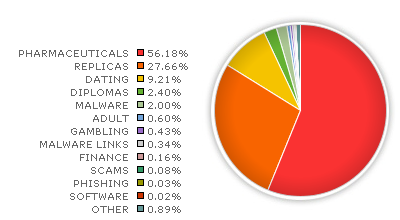
\includegraphics [height=5cm] {Imagens/m86security/spamtype.png}
			\caption {Distribuição do conteúdo de spam}
			\label{fig:spamtype}
		\end{figure}

		A distribuição de emissores de spam pelo mundo pode ser vista na Figura \ref{fig:spamworld}.

	\begin{figure}[ht]
		\begin{subfigure}[b]{\textwidth}
			\centering
			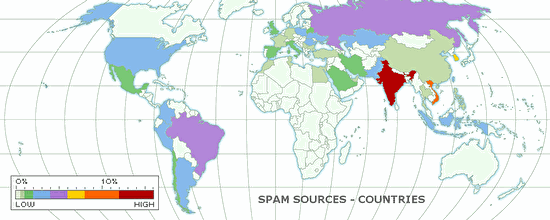
\includegraphics[height=5cm]{Imagens/m86security/spam-country-map.png}
			\caption{Mapa de emissores de spam((mude isso))}
		\end{subfigure}
		~
		\begin{subfigure}[b]{0.47\textwidth}
			\centering
			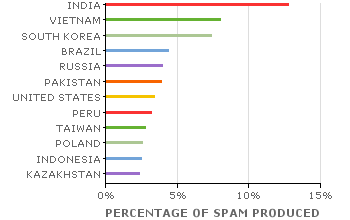
\includegraphics[height=5cm]{Imagens/m86security/spam-country-bar.png}
			\caption{12 países que mais emitem spam}
		\end{subfigure}
		~
		\begin{subfigure}[b]{0.47\textwidth}
			\centering
			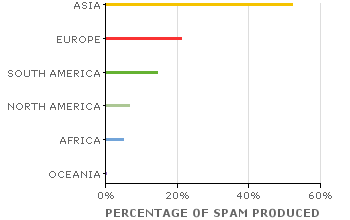
\includegraphics[height=5cm]{Imagens/m86security/spam-continent-bar.png}
			\caption{Percentual de spam emitido por continente}
		\end{subfigure}
		\caption{Emissão de spam no mundo}
		\label{fig:spamworld}
	\end{figure}

\newpage
\section{Filtros de Spam}
	Para acompanhar o aumento do número e da variedade de spams, vem sendo criados vários métodos para separar mensagens importantes de propagandas.
	São inúmeras as abordagens utilizadas. 
	Algumas se baseiam no \gls{cabecalho} da mensagem, outras na frequência das palavras utilizadas.
	Nas seções seguintes, serão brevemente discutidas algumas estratégias utilizadas no combate ao spam, e, como um exemplo, serão mostrados alguns dos filtros utilizados pelo \emph{Gmail}((citar?)).

	\subsection{Filtro baseado na estrutura do texto}
		Este tipo de filtro se baseia em cadeias específicas do cabeçalho do e-mail, como, por exemplo, a língua na qual foi escrito e o tipo do conteúdo da mensagem.

		Estes filtros podem ser facilmente criados pelos próprios usuários em grandes servidores de e-mail, e tem como objetivo não só detectar spam, mas também separar mensagens relevantes em categorias.

		A vantagem desta estratégia é o alto nível de personalização permitido, já que cada usuário pode criar seu próprio filtro dependendo do tipo de spam recebido. 
		Além disso, a probabilidade de haver falsos-positivos é menor, já que é o próprio usuário que escolhe os parâmetros de filtragem.
		
		Sua desvantagem é a possível necessidade de criação de vários filtros para se obter uma separação eficaz.


	\subsection{\emph{Whitelist}/Verificação}
		Uma abordagem mais agressiva para a filtragem de spam é a utilização de \emph{Whitelist} em conjunto com a verificação automática.

		Qualquer endereço que esteja nesta \emph{whitelist} tem sua mensagem enviada sem maiores problemas.
		Caso o endereço não esteja contido na lista, o \emph{\gls{mta}} envia uma mensagem de volta para o remetente, com instruções que, ao serem seguidas, adicionam o endereço do remetente na \emph{whitelist}.

		Como a maioria das mensagens de spam possui endereços de resposta falsos, as instruções não seriam seguidas e o e-mail não chegaria à caixa de entrada do destinatário.
		Caso o \emph{spammer} decida fazer o que lhe foi dito, ele será adicionado à lista, porém isso o torna mais facilmente rastreável.
		
		Apesar de ser uma maneira eficaz de diminuir os spams, ela pode prejudicar usuários legítimos que não podem ou querem atender a essa exigência, já que isso implicaria no não recebimento de sua mensagem.

		Como um exemplo deste tipo de abordagem, tem-se o \emph{Corlive.com}~\cite{corlive}, que é um servidor de e-mail que utiliza \emph{Captcha}~\cite{captcha} para validar os e-mails enviados e não permitir que \emph{bots} enviem spam.

	\subsection{Distribuição adaptativa de \emph{blacklist}}
		A \emph{blacklist} é formada por mensagens que foram classificadas como spam por usuários ou mesmo por endereços especiamente criados por servidores para atrair spam.

		Ao receber uma mensagem, o MTA utiliza um filtro por \emph{blacklist} para determinar se mesma é um spam conhecido, e ela só é enviada à caixa de entrada do destinatário caso ela não seja classificada como ilegítima.

		Esta estratégia se baseia no uso de técnicas estatísticas para sumarizar o conteúdo de um mensagem de forma que pequenas mutações no spam não impeçam seu reconhecimento.

		A probabilidade de haver falsos-positivos é pequena, já que é necessária uma marcação na mensagem para que ela entre na \emph{blacklist}. Além disso, quando ocorre uma marcação errônea de mensagens vastamente enviadas, como informativos, o gerenciador da lista pode desmarcá-las.
		
		Como é necessária a verificação da mensagem em um servidor, a performance deste método comparada a outros é baixa, sendo ele bastante lento.

		Um exemplo de software que implementa esta abordagem é o \emph{Pyzor}~\cite{pyzor}, um software implementado em \emph{Python} sob a licença \emph{GPL}.

	\subsection{Ranking baseado em regras}
		Este filtro possui regras de ranking, principalmente expressões regulares, e tenta fazer correspondências entre o padrão e a mensagem. 
		Cada equivalência adiciona ou diminui pontos da mensagem.
		
		Se a quantidade de pontos do e-mail exceder um determinado threshold, é classificado como spam, caso contrário, é classificado como uma mensagem legítima.

		A dificuldade deste tipo de filtro é que, apesar de existirem regras que são contantes com o decorrer do tempo, como endereço de resposta falso ou áudio como tipo de conteúdo, há outras que mudam com o tempo, como os produtos dos quais os spams fazem propaganda, e isso causa a necessidade constante de atualização das regras.

		Um software que implementa este tipo de filtro é o \emph{SpamAssassin}~\cite{spamassassin}, um projeto open-source da \emph{Apache}.

	\subsection{Filtro Bayesiano}
		A abordagem do filtro Bayesiano, criado por Paul Graham, é a utilização de modelos Bayesianos de probabilidade para determinar se uma mensagem é legítima ou não.

		É criado um dicionário de palavras contendo a probabilidade de ela estar em um spam e a probabilidade de estar em uma mensagem válida. Esse dicionário é utilizado para calcular a probabilidade geral de a mensagem ser um spam, com base na teoria da probabilidade condicional de Bayes.

		Este filtro possui traz vários benefícios como ser automatizável, ou seja, não são necessárias pessoas para definir os valores de probabilidade, já que ele pode aprender, isto é, adicionar novas palavras ou modificar a probabilidade de uma palavra de acordo com a marcação de um e-mail como spam ou válido.

		Além disso, sua implementação e a teoria em que se baseia são extremamente simples e sua performance é melhor que a de filtros baseados em regras.
		
		Um software que implementa o filtro Bayesiano é o \emph{SpamBayes}~\cite{spambayes}, disponível para os serviços de e-mail \emph{Gmail}, \emph{MSN Hotmail}, \emph{Yahoo! Mail}, entre outros.

	\subsection{Filtro Markoviano}
		O filtro Markoviano é um filtro estatístico baseado na teoria de \glspl{cadmarkov}~\cite{markov}, e leva em consideração a probabilidade de transição entre uma palavra e outra, ou seja, dada uma palavra, ele tenta predizer qual é a próxima.

		Diferentemente do filtro Bayesiano, que é baseado em palavras independentes, o filtro Markoviano trabalha em cima de frases, e por isso, seu desempenho tende a ser maior, já que utiliza uma abordagem holística do texto.
		
	Esta estratégia é utilizada no filtro de spam \gls{crm114}, juntamente com outras abordagens que não serão discutidas neste trabalho. Seu desempenho foi testado para diferenciar documentos japoneses confidenciais de não confidenciais, e a acurácia obtida foi maior que $99\%$ e taxa de falsos-positivos foi menor que $5.3\%$~\cite{fmarkov:japtest}.

	\subsection{Gmail}
		Uma das técnicas utilizadas pelo provedor de serviço de correio eletrônico \emph{Gmail} é o aprendizado baseado em instâncias, chamado pelo provedor de \emph{Community clicks}, em que os filtros de spam usados para todos os usuários são modificados a cada mensagem que um usuário marca como spam ou como mensagem legítima.

		Outra técnica é o aprendizado de máquina usado para combinar e indexar os conjuntos de busca do buscador Google, que permite a junção de vários fatores para identificar mensagens semelhantes e classificá-las como spam.
		Além disso, são aplicadas ferramentas como \emph{OCR} de outro serviço da empresa, o \emph{Google Book Search}, serviço de busca em livros (podem ser imagens), para identificar spams em forma de imagens.

		A filtragem pode feita por endereço, ou seja, se um usuário marca a mensagem de um emissor como spam várias vezes, próximas mensagens enviadas por esse endereço irão para a caixa de spam automaticamente, como um filtro por distribuição de blacklist.

		Além disso, sempre é checado se o endereço do remetente é autenticado por meio de órgãos autenticadores para tentar impedir golpes de \emph{phishing}.
		Entretanto, não ter um certificado não é suficiente para a mensagem ser marcada como spam.
		Esta checagem é feita como parte da filtragem e é combinada com denúncias de usuários e outras técnicas.

		O \emph{Gmail} também permite a criação personalizada de fitros de spam baseados em regras, de acordo com os seguintes campos do e-mail: remetente, destinatário, assunto e corpo da mensagem. 
		É possível, ainda, filtrar pela presença ou ausência de palavras, utilizar operadores lógicos como \emph{e}, \emph{ou} e \emph{não}, e denotar ``qualquer um'' por meio de \emph{*}.

		Com todo esse leque de ferramentas, a filtragem feita pelo serviço de correio eletrônico do gigante buscador é bastante interessante e a melhora de sua eficácia pode ser vista na Figura \ref{gmail:chart}.

		\begin{figure*}[ht]
			\centering
			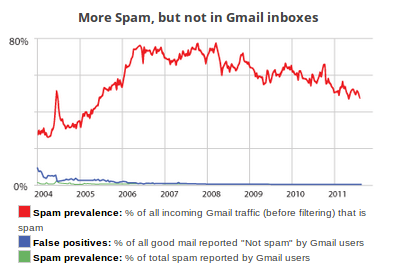
\includegraphics[height=7cm]{Imagens/gmail/spamchart.png}
			\caption{Percentual de filtragem ao longo dos anos}
			\label{gmail:chart}
		\end{figure*}

\newpage
\section{Casos Reais}
	Nas próximas subseções, são apresentados casos reais de como o spam afeta o cotidiano das pessoas.

	\subsection {Coxinha na promoção}
		A colunista Lúcia Guimarães do jornal \emph{Estadão} recebeu uma notificação de uma promoção de uma coxinha bo Boteco do Joaquim, na Cidade Baixa em Porto Alegre.
		O salgado, um espeto de ``Coxinha de Asa'', custava $R\$12,50$ e, com um desconto de aproximadamente $50\%$, passou a custar $R\$6,00$.

		A notificação da promoção para Lúcia foi feita via e-mail e ela gostaria de aproveitar a promoção, se pudesse.
		O comentário feito por Lúcia sobre o e-mail pode ser visto à seguir.

		``Foi o Boteco do Joaquim que avisou esta guria da promoção. E concluo a afirmação no tom agudo de uma interrogação, como fazem os gaúchos. Uma pena que não posso economizar $R\$ 6,50$ num almoço porque a passagem daqui para o Boteco custa $R\$ 4$ mil.''

		Como se pode perceber, a escritora não mora em Porto Alegre.
		Na verdade, sua atual moradia é em Nova Iorque e, ainda assim, ela recebe e-mails com propagandas de coxinhas da Cidade Baixa.

		((Ligar))

		``Se alguma corporação estiver espionando minha correspondência eletrônica com base num algoritmo, pode montar um perfil em que: 
		Eu como coxinha em Porto Alegre; 
		corto o cabelo em Belo Horizonte; 
		compro câmeras no Estado do Maine; 
		passo os fins de semana em Búzios; 
		encomendo pornografia do Estado de Nevada. 
		Enfim, sou uma verdadeira cidadã do mundo, cheia de caprichos e perversões.''
			
		O que se pode concluir a partir deste caso é que o objetivo do Boteco do Joaquim foi atingido, já que a jornalista leu o e-mail e compraria a coxinha se conseguisse, porém a propaganda poderia ser enviada de forma mais inteligente somente para potenciais consumidores, categoria na qual Lúcia não se inclui.

	\subsection {Spam cria amizades no mundo}
		Um \emph{spammer} indiano enviou um e-mail escrito em 
\newpage
\section{Estudo de Caso}
	O estudo de caso apresentado à seguir é baseado em fatos, mas não é completamente real. 

	\subsection{Contexto}	
    Juliano, professor de uma universidade renomada, ficou responsável por ministrar uma disciplina em um determinado semestre e delegou a tarefa de auxiliá-lo (como monitor bolsista) a Eduardo. 
	Eduardo, por sua vez, é pós-graduando sob a tutoria de Juliano e está na iminência de defender sua tese de mestrado.

    A média final da disciplina ministrada é composta por projetos (para serem feitos em grupos) de complexidade média e por nenhuma prova.
	Os projetos são lançados ao longo do semestre e cada um deles fica responsável por cobrir parte do conteúdo programático.

	Durante a realização do projeto, é necessário fazer vários testes para comprovar a eficiência da implementação. 
	Os testes devem ser feitos em máquinas específicas fornecidas pela instituição.
	
	Como as máquinas são compartilhadas por todos os grupos e ocorriam testes simultâneos, havia flutuações indesejadas nos resultados obtidos.
	Por isso, após várias reclamações, o professor decidiu alocar períodos de tempo reservados para cada grupo, de forma que outros grupos seriam penalizados caso utilizassem os recursos em um período que não fosse seu.

	Foi feita uma alocação inicial, escolhida por Juliano, porém os horários não levavam em conta a disponibilidade dos alunos. 
	Por isso, havia grupos que não estavam livres durante seu período, o que levou vários a enviarem e-mails ao professor para pedir que a alocação fosse modificada.
	Além disso, houve grupos que não conseguiram terminar seus testes na sua vez e pediram mais tempo para o professor.

	Juliano decidiu atender ao pedido dos alunos e disse para Eduardo mandar um e-mail aos alunos para avisar todas as mudanças feitas.
	
	Eduardo fez como lhe foi dito e enviou e-mails a todos os alunos matriculados na disciplina, avisando sobre as modificações e extensões nos horários.
	Entretanto, após alguns envios, percebeu que ainda aconteceriam várias modificações e que isso geraria uma grande quantidade de mensagens enviadas que não eram importantes para todos os alunos, como, por exemplo, os alunos que já haviam realizado os testes de forma bem sucedida.

	Era possível utilizar o \emph{site} da disciplina para avisar sobre as modificações, assim como foi feito para a primeira alocação. 
	O problema é que somente o professor poderia fazê-lo, e Juliano não parecia disposto a gastar seu tempo de pesquisa para atualizar o documento que continha os horários reservados.

	Havia, ainda, a possibilidade de enviar o aviso somente para os grupos influenciados pela modificação, mas isso seria mais trabalhoso do que a primeira opção, já que Juliano ou Eduardo teriam que escolher para quem mandariam a mensagem.
	
	Eduardo sabia que se mandasse os e-mails, vários alunos ficariam insatisfeitos e isso poderia ser considerado spam e disse isso a Juliano, que respondeu ser irrelevante.

	O orientando não queria irritar seu orientador às vésperas de sua defesa, já que isso poderia prejudicá-lo. 
	Por outro lado, se estivesse no lugar dos alunos, se sentiria incomodado pelo spam acadêmico recebido.

\newpage
	\subsection{Dados Relevantes}
		No caso estudado, são as partes envolvidas são:
		\begin{itemize}
			\item Juliano, professor, orientador de Eduardo e pesquisador da universidade;
			\item Eduardo, mestrando, monitor da disciplina e orientando de Juliano;
			\item Alunos que cursam a disciplina ministrada por Juliano e monitorada por Eduardo. 
		\end{itemize}

		As obrigações das partes envolvidas para com as outras são dadas na Tabela \ref{tab:obrig} e na Figura \ref{fig:obrig}.

		\begin{table}[h!]
			\centering
			\begin{tabular}{@{\extracolsep{\fill}}l C{0.15\textwidth} C{0.15\textwidth} C{0.15\textwidth}}
				\hline
									&	Juliano		&	Eduardo	&	Alunos\\	
				\hline
				Juliano	&	Pesquisar	&	Orientar para a docência	&	Passar conhecimento\\
				\hline
				Eduardo	&	Obedecer \linebreak \linebreak Auxiliar na disciplina	&	Prezar pela \linebreak pós-graduação	&	Avisar sobre \linebreak mudanças\\
				\hline
			Alunos	&	Ser aprovado na disciplina	&			&	Manter boas notas\\
				\hline
			\end{tabular}
			\caption {Tabela de obrigações}
			\label{tab:obrig}
		\end{table}
		~
		\begin{figure}[h!]
			\centering
			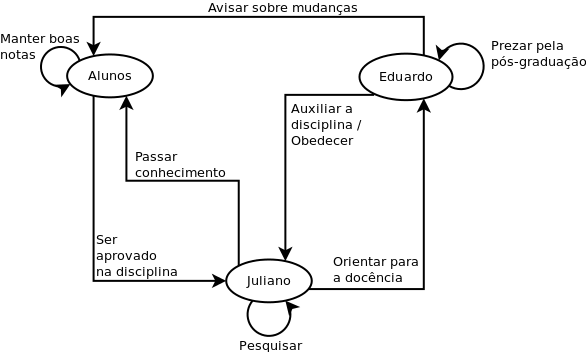
\includegraphics[height=7cm]{diagramas/grafo-de-obrigacoes.png}
			\caption{Grafo de obrigações}
			\label{fig:obrig}
		\end{figure}

		As alternativas de decisão de Eduardo são:
		\begin{itemize}
			\item Insistir para Juliano modificar o documento no \emph{site};
			\item Enviar e-mails sobre as modificações somente para os alunos influenciados pelas mudanças feitas (componentes dos grupos);
			\item Enviar e-mails de todas as modificações a todos os alunos matriculados;
			\item Guardar as modificações e enviá-las somente uma vez para todos os alunos.
		\end{itemize}
	
	\subsection{Códigos de ética da ACM violados}
		Os códigos da ACM violados são os seguintes:
		\begin{itemize}
			\item ``Contribuir para o bem-estar humano e da Sociedade''\\
				Se Eduardo enviar e-mails a todos os alunos sobre as modificações, os alunos não interessados se sentirão incomodados.
				Além disso, Juliano corre o risco de atribuir horários inconsistentes por não possuir todas as informações de forma organizada;
			\item ``Procurar alcançar a maior qualidade, eficácia de dignidade tanto nos processos como nos produtos do trabalho profissional''\\
				Se Eduardo enviar e-mails sobre as notificações, os alunos interessados, Eduardo e Juliano perderão tempo por ter que buscar as modificações em sua caixa de e-mail.
				Além disso, Juliano corre o risco de atribuir horários inconsistentes por não possuir todas as informações de forma organizada;
			\item ``Adquirir e manter competência profissional''\\
				((TODO))
				
		\end{itemize}

	\subsection{Potenciais benefícios e vulnerabilidades}
		Os potenciais benefícios de cada solução são dados na Tabela \ref{tab:ben} e as potenciais vulnerabilidades são dadas na Tabela \ref{tab:vul}.

		Os alunos foram divididos em dois grupos: alunos interessados e alunos não interessados.
		O primeiro grupo é composto pelos alunos relacionados às modificações, enquanto o segundo é composto pelos outros.
		\begin{table}[h!]
			\centering
			\begin{tabular}{@{\extracolsep{\fill}}C{0.15\textwidth}  C{0.15\textwidth} C{0.15\textwidth} C{0.15\textwidth} C{0.15\textwidth} C{0.15\textwidth}}
				\hline
				 & \textbf{Insistir para Juliano modificar no site} & \textbf{Enviar apenas para os interessados} & \textbf{Enviar para todos} & \textbf{Enviar todas as modificações de uma vez}\\
				\hline
				Alunos interessados & Não receberão nenhum e-mail \linebreak \linebreak Serão notificados & Serão notificados & Serão notificados & Receberão menos e-mails \linebreak \linebreak Serão notificados\\
				\hline
				Alunos não interessados & Não receberão nenhum spam & Não receberão nenhum spam &  & Receberão menos e-mails\\
				\hline
				Eduardo & Não precisa enviar os e-mails & & & Envia menos e-mails \\
				\hline
				Juliano & & Não envia e-mails & Não envia e-mails & Não envia e-mails \\
				\hline
			\end{tabular}
			\caption{Tabela de benefícios potenciais}
			\label{tab:ben}
		\end{table}
		~
		\begin{table}[h!]
			\centering
			\begin{tabular}{@{\extracolsep{\fill}}C{0.15\textwidth} C{0.15\textwidth} C{0.15\textwidth} C{0.15\textwidth} C{0.15\textwidth}}
				\hline
				& \textbf{Insistir para Juliano modificar o documento no site} & \textbf{Enviar apenas para os interessados} & \textbf{Enviar para todos} & \textbf{Enviar todas as modificações de uma vez}\\
				\hline
				Alunos interessados & & & Recebe spam & Recebe spam \\
				\hline
				Alunos não interessados & & & Recebe spam & Recebe spam \\
				\hline
				Eduardo & & Envia e-mails & Envia e-mails & Envia e-mails \\
				\hline
				Juliano & Precisa modificar o documento & & &\\
				\hline
			\end{tabular}
			\caption{Tabela de vulnerabilidades potenciais}
			\label{tab:vul}
		\end{table}
		~
		\begin{table}
			\begin{tabular*}{\textwidth}{@{\extracolsep{\fill}} C{0.117\textwidth} | C{0.117\textwidth} C{0.117\textwidth} C{0.117\textwidth} C{0.117\textwidth} C{0.117\textwidth} C{0.117\textwidth}}
				\cline{2-7}
				& & & \textbf{Insistir para Juliano modificar no site} & \textbf{Enviar apenas para os interessados} & \textbf{Enviar para todos} & \textbf{Enviar todas as modificações de uma vez}\\
				\hline
				\multirow{3}{*}{Eduardo}  & Para ele mesmo & Prezar pela pós-graduação & - - & - - & - & - \\
				\cline{2-7}
						& Juliano & Obedecer & - & + & + + & + \\
				\cline{2-7}
						& Alunos & Notificar & + - & + & + & + \\
				\hline
				Juliano & Para ele mesmo & Pesquisar & - - &  &  & \\
				\hline
			\end{tabular*}
			\caption{Tabela de obrigações afetadas}
		\end{table}
		
	\subsection{Análise das possíveis decisões}
		Pelas tabelas acima, é possível observar que qualquer decisão que não seja a de modificar o documento no \emph{site} é igualmente boa.

		Já para os alunos interessados, como seu objetivo é ser notificados, todas as alternativas são boas, porém a melhor seria que eles só recebam e-mails sobre seu grupo.
		A opção de enviar todas as atualizações de uma vez pode não ser vantajosa, pois os grupos ficarão em dúvida se seu pedido foi concedido até que a mensagem seja enviada.

		Para os alunos não interessados, as alternativas nas quais eles não recebem spam são ótimas, ou seja, modificar o documento ou enviar e-mails somente para os interessados.

		Por fim, para Eduardo, a melhor opção é Juliano fazer as atualizações, já que Eduardo não terá que incomodar os alunos ou enviar e-mails.
		Entre as demais, a pior seria ter que enviar e-mails para cada grupo dependendo da modificação, por tomar um tempo que ele poderia estar dedicando ao seu mestrado.

	\subsection{Decisão consensual}
		A melhor opção seria Eduardo tentar convencer Juliano a fazer as atualizações no \emph{site}.
		Entretanto, se Eduardo perceber que isso afetará muito negativamente sua relação com o orientador e que seu mestrado poderá ser prejudicado, Eduardo pode juntar várias modificações e enviar em um bloco.
		
\newpage
\section{Conclusão}

\newpage
\printglossaries
\addcontentsline{toc}{section}{Glossário}

\newpage
\bibliography{refs}
\bibliographystyle{acm}
\addcontentsline{toc}{section}{Referências}

%\newacronym{acm}{ACM}{Association for Computing Machinery}
\newglossaryentry{email} {
	name={E-mail}, 
	description={Correio eletrônico, termo usualmente utilizado para denotar a mensagem eviada por este meio.}
}
\newglossaryentry{cabecalho} {
	name={cabeçalho}, 
	description={Parte do e-mail que contem informações suplementares de transmissão. Entre seus campos, são encontrados endereço do emissor, endereço do receptor, endereço de resposta, data de emissão, tipo do conteúdo e assunto.}
}
\newglossaryentry{falsopos} {
	name={falso-positivo}, 
	description={Classificação errônea na qual, para este contexto, um e-mail legítimo é classificado como spam}
}
\newglossaryentry{captcha} {
	name={CAPTCHA}, description={\emph{Completely Automated Public Turing test to tell Computers and Humans Apart}. Teste criado para diferenciar seres humanos de máquinas. Consiste em imagens de mensagens distorcidas para evitar a interpretação automática por máquinas.}
}
\newglossaryentry{spambot} {
	name={spambot},
	description={Bot projetado para enviar spam de forma massiva, automaticamente.}
}
\newglossaryentry{bot} {
	name={bot}, 
	description={Softwares criados para realizar alguma tarefa de forma automatizada.}
}
\newglossaryentry{cadmarkov} {
	name={Cadeia de Markov}, description={Conjunto de estados no qual um processo ocorre. O processo inicia em um estado e se move sucessivamente, transicionando entre estados, a cada passo. O estado para o qual o processo se move depende unicamente, de forma probabilística, do estado em que ele se encontra atualmente.}
}
\newglossaryentry{crm114} {
	name={\emph{CRM114}, 
	description={Software anti-spam baseado em técnicas estatísticas para a filtragem e classificação de dados. Seu código fonte na linguagem C é disponibilizado sob a licença \emph{GPL}}}
}
\newglossaryentry{gpl} {
	name={\emph{GPL}, 
	description={\emph{General Public License}. Licença para software livre.}}
}
\newglossaryentry{whitelist} {
	name={whitelist}, 
	description={Lista de endereços de e-mail de remetentes legítimos, previamente validados.}
	}
\newglossaryentry{blacklist} {
	name={blacklist}, 
	description={Lista de mensagens classificadas como spam.}
	}
\newacronym{mta}{MTA}{Mail Transfer Agent}{
	description={Software que transfere mensagens de correio eletrônico de um cliente para outro, baseado em uma arquitetura cliente-servidor.}
}
\newglossaryentry{threshold} {
	name={threshold}, 
	description={Valor utilizado como limitante para uma classificação.}
}


\end{document}
